

The deuteron is the simplest composite nuclear system, and in many ways it is as important to understanding bound states in QCD as the hydrogen atom was to understanding bound systems in QED.  Our experimental and theoretical understanding of the deuteron remains unsatisfying. By taking a ratio of electron scattering off of tensor-polarized and unpolarized deuterons, the S- and D-wave states can be disentangled, leading to a fuller understanding of the repulsive nucleon core. 

Understanding the nucleon-nucleon potential of the deuteron is essential for understanding short-range correlations. To resolve the short-range structure of nuclei on the level of nucleon and hadronic constituents, we need processes that transfer to the nucleon constituents both energy and momentum larger than the scale of the NN short range correlations. By scanning over a large range of $Q^2$, we can measure how these processes begin to dominate the tensor asymmetry $A_{zz}$.



%Jefferson Lab is the ideal place to investigate tensor structure in a deuteron target at intermediate and large $x$.  We describe such a measurement in this proposal.

\subsection{Deuteron Wavefunction}


\subsection{Tensor Asymmetry Azz}


The S- and D-states are to the tensor asymmetry $A_{zz}$ by~\cite{Frankfurt:1988nt}
\begin{equation}
	A_{zz} \propto \frac{u(k)w(k)\sqrt{2}+\frac{1}{2}w^2(k)}{u^2(k)+w^2(k)},
\end{equation}
where $u(k)$ is the $^3S_1$ wave function and $w(k)$ is the $^3D_1$ wave function.


For decades~\cite{PhysRev.81.165}, it has been known that the nucleon-nucleon potential has a short-range repulsive core, which is responsible for the stability of strongly interacting matter. However, a description of the repulsive core remains largely unconstrained and our understanding of QCD dynamics at short distances ($\leq 0.5\mathrm{~fm}$) largely incomplete~\cite{Sargsian:2014bwa}. 

Due to their small size~\cite{needed} and simple structure, tensor polarized deuterons are ideal for studying nucleon-nucleon interactions. Tensor polarization enhances the D-state wavefunction, which compresses the deuteron from $\sim?\mathrm{~fm}$ to $\sim0.5\mathrm{~fm}$~\cite{Forest:1996kp} and has been noted to be revealing of short-range QCD effects.

\begin{figure}
\centering
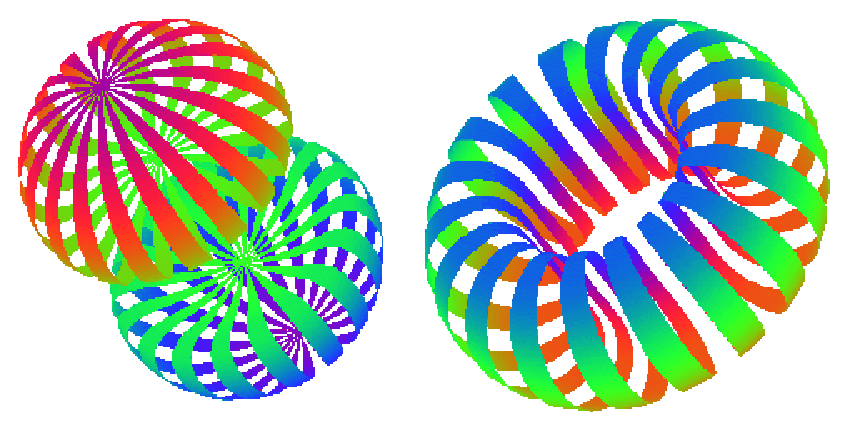
\includegraphics[width=0.5\textwidth]{figs/deuteron_states.eps}
\caption{\label{fig:deuteron}
Equidensity lines of the deuteron in its two spin projections, $M_J=\pm 1$ and $M_J=0$, respectively.
{\it Reproduced from~\cite{Carlson:1997qn,Forest:1996kp}}.
}
\end{figure}

